

\tikzset{every picture/.style={line width=0.75pt}} %set default line width to 0.75pt        

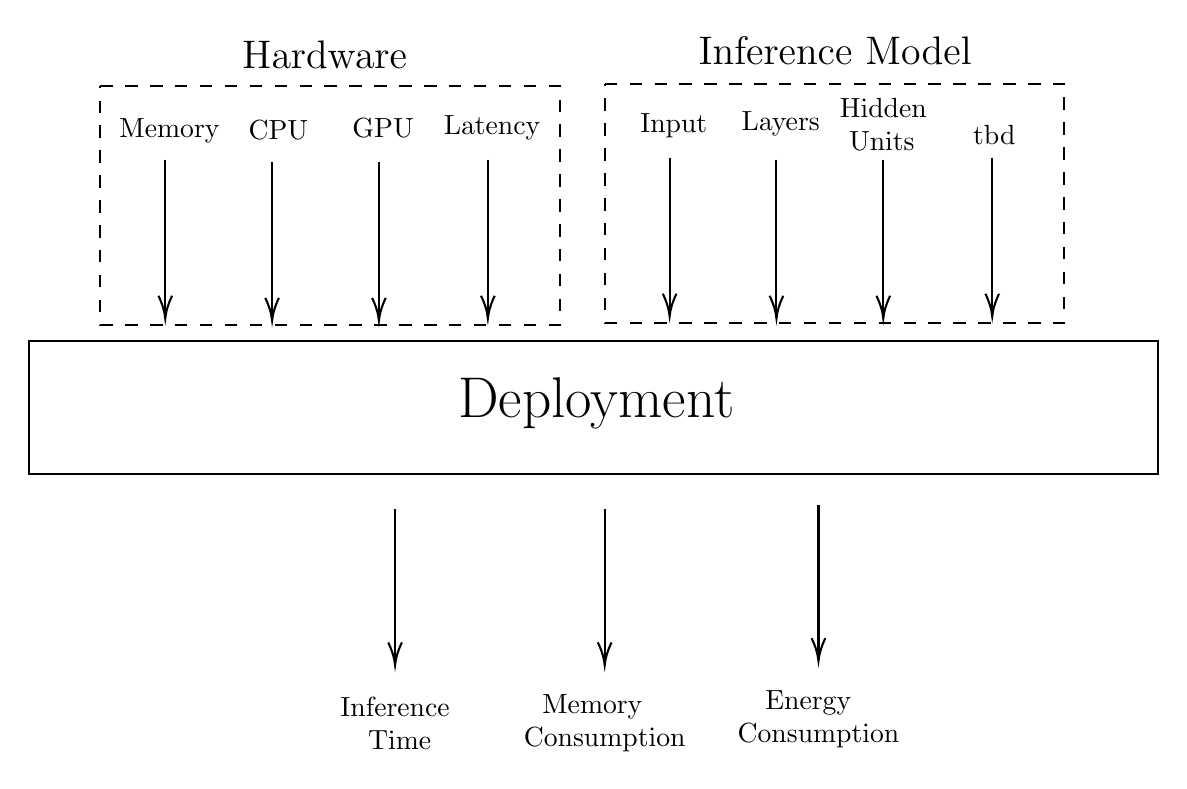
\begin{tikzpicture}[x=0.75pt,y=0.75pt,yscale=-1,xscale=1]
%uncomment if require: \path (0,556); %set diagram left start at 0, and has height of 556

\draw   (99.5,235) -- (643.5,235) -- (643.5,299) -- (99.5,299) -- cycle ;
\draw    (165.29,147.5) -- (165.29,221.98) ;
\draw [shift={(165.29,223.98)}, rotate = 270] [color={rgb, 255:red, 0; green, 0; blue, 0 }  ][line width=0.75]    (10.93,-3.29) .. controls (6.95,-1.4) and (3.31,-0.3) .. (0,0) .. controls (3.31,0.3) and (6.95,1.4) .. (10.93,3.29)   ;

\draw    (216.76,148.52) -- (216.76,223) ;
\draw [shift={(216.76,225)}, rotate = 270] [color={rgb, 255:red, 0; green, 0; blue, 0 }  ][line width=0.75]    (10.93,-3.29) .. controls (6.95,-1.4) and (3.31,-0.3) .. (0,0) .. controls (3.31,0.3) and (6.95,1.4) .. (10.93,3.29)   ;

\draw    (268.23,148.52) -- (268.23,223) ;
\draw [shift={(268.23,225)}, rotate = 270] [color={rgb, 255:red, 0; green, 0; blue, 0 }  ][line width=0.75]    (10.93,-3.29) .. controls (6.95,-1.4) and (3.31,-0.3) .. (0,0) .. controls (3.31,0.3) and (6.95,1.4) .. (10.93,3.29)   ;

\draw    (320.72,147.5) -- (320.72,221.98) ;
\draw [shift={(320.72,223.98)}, rotate = 270] [color={rgb, 255:red, 0; green, 0; blue, 0 }  ][line width=0.75]    (10.93,-3.29) .. controls (6.95,-1.4) and (3.31,-0.3) .. (0,0) .. controls (3.31,0.3) and (6.95,1.4) .. (10.93,3.29)   ;

\draw  [dash pattern={on 4.5pt off 4.5pt}] (134,112) -- (355.5,112) -- (355.5,227) -- (134,227) -- cycle ;
\draw    (408.29,146.5) -- (408.29,220.98) ;
\draw [shift={(408.29,222.98)}, rotate = 270] [color={rgb, 255:red, 0; green, 0; blue, 0 }  ][line width=0.75]    (10.93,-3.29) .. controls (6.95,-1.4) and (3.31,-0.3) .. (0,0) .. controls (3.31,0.3) and (6.95,1.4) .. (10.93,3.29)   ;

\draw    (459.76,147.52) -- (459.76,222) ;
\draw [shift={(459.76,224)}, rotate = 270] [color={rgb, 255:red, 0; green, 0; blue, 0 }  ][line width=0.75]    (10.93,-3.29) .. controls (6.95,-1.4) and (3.31,-0.3) .. (0,0) .. controls (3.31,0.3) and (6.95,1.4) .. (10.93,3.29)   ;

\draw    (511.23,147.52) -- (511.23,222) ;
\draw [shift={(511.23,224)}, rotate = 270] [color={rgb, 255:red, 0; green, 0; blue, 0 }  ][line width=0.75]    (10.93,-3.29) .. controls (6.95,-1.4) and (3.31,-0.3) .. (0,0) .. controls (3.31,0.3) and (6.95,1.4) .. (10.93,3.29)   ;

\draw    (563.72,146.5) -- (563.72,220.98) ;
\draw [shift={(563.72,222.98)}, rotate = 270] [color={rgb, 255:red, 0; green, 0; blue, 0 }  ][line width=0.75]    (10.93,-3.29) .. controls (6.95,-1.4) and (3.31,-0.3) .. (0,0) .. controls (3.31,0.3) and (6.95,1.4) .. (10.93,3.29)   ;

\draw  [dash pattern={on 4.5pt off 4.5pt}] (377,111) -- (598.5,111) -- (598.5,226) -- (377,226) -- cycle ;
\draw    (377,315.95) -- (377,389) ;
\draw [shift={(377,391)}, rotate = 270] [color={rgb, 255:red, 0; green, 0; blue, 0 }  ][line width=0.75]    (10.93,-3.29) .. controls (6.95,-1.4) and (3.31,-0.3) .. (0,0) .. controls (3.31,0.3) and (6.95,1.4) .. (10.93,3.29)   ;

\draw    (480,313.95) -- (480,387) ;
\draw [shift={(480,389)}, rotate = 270] [color={rgb, 255:red, 0; green, 0; blue, 0 }  ][line width=0.75]    (10.93,-3.29) .. controls (6.95,-1.4) and (3.31,-0.3) .. (0,0) .. controls (3.31,0.3) and (6.95,1.4) .. (10.93,3.29)   ;

\draw    (276,315.95) -- (276,389) ;
\draw [shift={(276,391)}, rotate = 270] [color={rgb, 255:red, 0; green, 0; blue, 0 }  ][line width=0.75]    (10.93,-3.29) .. controls (6.95,-1.4) and (3.31,-0.3) .. (0,0) .. controls (3.31,0.3) and (6.95,1.4) .. (10.93,3.29)   ;


\draw (373,265) node  [align=left] {{\huge Deployment}};
\draw (167.31,133.32) node  [align=left] {Memory};
\draw (219.78,133.34) node  [align=left] {CPU};
\draw (270.25,132.34) node  [align=left] {GPU};
\draw (322.73,132.34) node  [align=left] {Latency};
\draw (410.31,131.32) node  [align=left] {Input};
\draw (461.78,130.34) node  [align=left] {Layers};
\draw (511.25,130.34) node  [align=left] {Hidden\\ \ Units};
\draw (564.73,135.34) node  [align=left] {tbd};
\draw (242,97) node  [align=left] {{\Large Hardware}};
\draw (488,95) node  [align=left] {{\Large Inference Model}};
\draw (276,419) node  [align=left] {Inference \\ \ \ \ Time};
\draw (377,419) node  [align=left] { \ \ Memory\\Consumption};
\draw (480,417) node  [align=left] { \ \ \ Energy\\Consumption};


\end{tikzpicture}
